\section{Architectural Design}
	\subsection{Overview}
	In this section we will talk about the system in its complex. We will show how we think that it should
	work, in particular we will present which should be its structure, the most important components and
	how they interact each other. We thought our system with a four tier architecture, in order to be compatible
	with a JEE Architecture implementation.
	\begin{figure}[h!]
		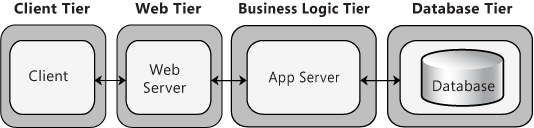
\includegraphics[width=\linewidth]{../SE2_IMAGES/4tier}
		\caption{Four tier architecture}
	\end{figure}
	\newline
	However, we do not want to limit the ways it could be implemented, so
	we will present the JEE as an example, \textbf{not as a constraint}. JEE is useful because provides some services
	"on the shelf" (ready to use) and we recommend to reuse the existing code to avoid a useless waste of time,
	but the possibility is always open for a more specific, and performing, implementation of the system.
	\clearpage
	\begin{figure}[h!]
		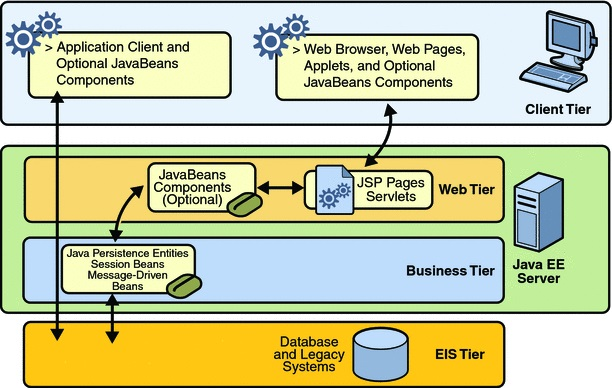
\includegraphics[width=\linewidth]{../SE2_IMAGES/jee}
		\caption{Java Enterprise Edition architecture}
	\end{figure}
	\begin{description}
		\item[Client tier] contains Application Clients and Web Browsers and it is the layer that interacts
		directly with the actors. In our case this tier contains both of them, because we have a usual web
		application and a mobile app.
		\item[Web tier] contains the Servlets and Dynamic Web Pages that needs to be elaborated. It could
		also include some optional JavaBeans. This tier receives the requests from the client tier and forwards
		the pieces of data collected to the business tier waiting for processed data to be sent
		to the client tier correctly formatted
		\item[Business tier] contains the Java Beans (the business logic of the application)	and Java
		Persistence Entities which represent the physical data of the system.
		\item[EIS tier] contains the persistent data source and destination.	It is another way to refer
		to the database of our system.
	\end{description}
	\newpage
	\subsection{High Level Components and their interaction}
	\begin{figure}[h!]
		\begin{center}
			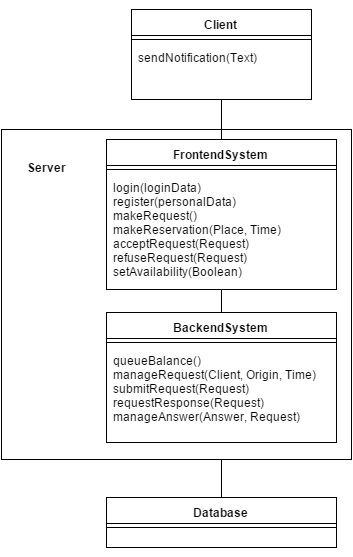
\includegraphics[height=0.5\textheight]{../SE2_IMAGES/HLC}
			\caption{High Level Component representation}
		\end{center}
	\end{figure}
	\newpage
	\begin{landscape}
	\subsection{Component view}
		\begin{figure}[h!]
			\begin{center}
				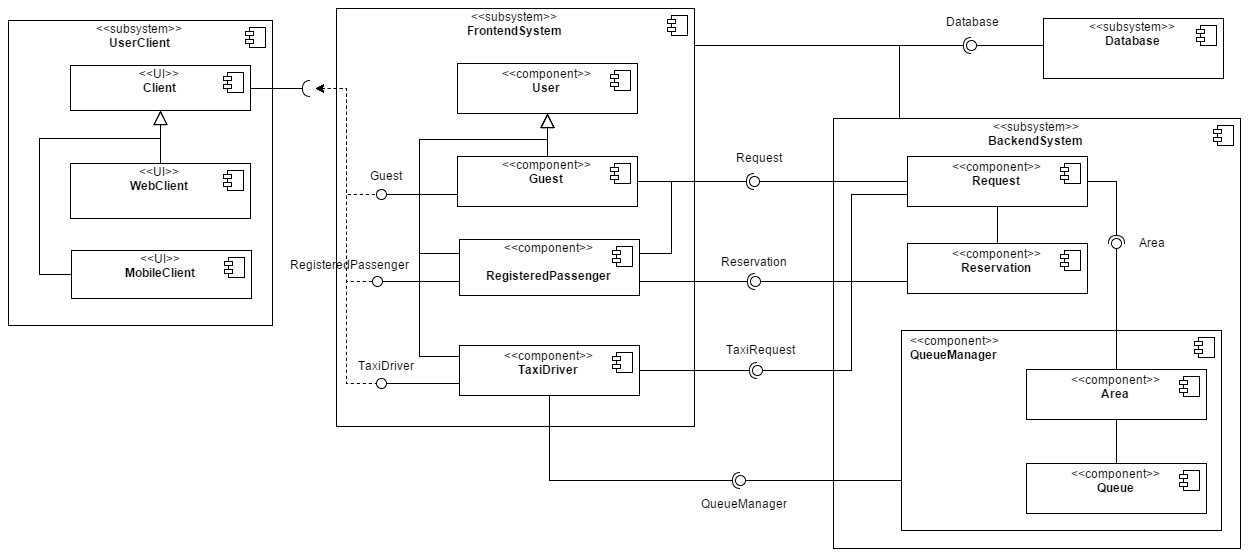
\includegraphics[width=0.9\linewidth]{../SE2_IMAGES/ComponentDiagram}
				\caption{Component Diagram}
			\end{center}
		\end{figure}
	\end{landscape}
	\newpage
	\subsubsection{Backend}
		\begin{figure}[h!]
			\begin{center}
				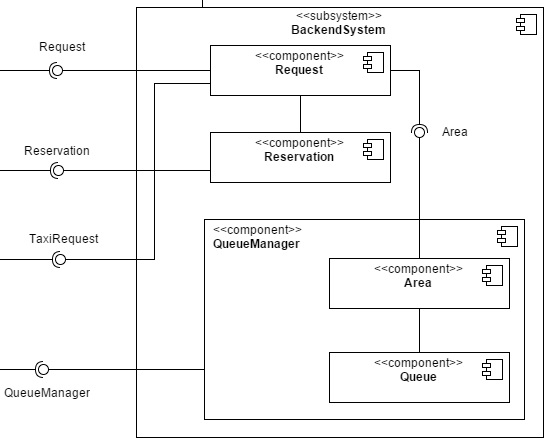
\includegraphics[width=1\linewidth]{../SE2_IMAGES/Backend}
				\caption{Backend components}
			\end{center}
		\end{figure}
		In this subsystem we have placed all the components (mainly entities) that we do not want to let the client
		interact directly. It is in direct communication with the frontend, responsible of the user
		management, and the database. This is practically the core of our system.
		\paragraph{Request}
		This is a stateful component. A User (Guest or RegisteredPassenger) can ask to create an instance
		which will be strictly related to the User himself and to the TaxiDriver who is asked to satisfy the
		request. A record in the database will be created to keep track of the operation, but when a taxi
		driver accepts or when the user closes the session, the request has no sense to exist anymore.
		In case a request is created automatically by a reservation, it will be related to the same user that booked it.
		\paragraph{Reservation}
		This is a stateful component. A RegisteredPassenger can ask to create an instance
		which will be strictly related to the User himself. A record in the database will be created to
		keep track of the operation, but when the User closes his session, the reservation has no sense to exist
		anymore. At the right time a job will be launched, creating a Request (even if the original instance
		does not exist anymore, the informations are stored in the database).
		\paragraph{QueueManager}
		This is a singleton component. Its interface is used by all the taxi drivers to interact with the areas and
		the queues. It is also responsible for the maintenance and the balancing of the queues.
		\paragraph{Area}
		This component is stateless. It is not connected to a single User, but, simply because it represents an Area,
		it has to serve all the users that require that area in the same way, there is no reason to relate the
		life of an area to the user's one. The main goal of this component is to manage the access to the one and
		only queue it contains.
		\paragraph{Queue}
		This is not truly an independent component, because we want to keep it strictly connected to the area,
		but we also want to be able to manage it without passing through the Area component all the times.
		It is easier fort he QueueManager to operate with a direct access to the queues.
		It is also sometimes useful to go back to areas from queues, so we keep a two way connection between them.
	\begin{landscape}
	\subsection{Deployment view}
		\begin{figure}[h!]
			\begin{center}
				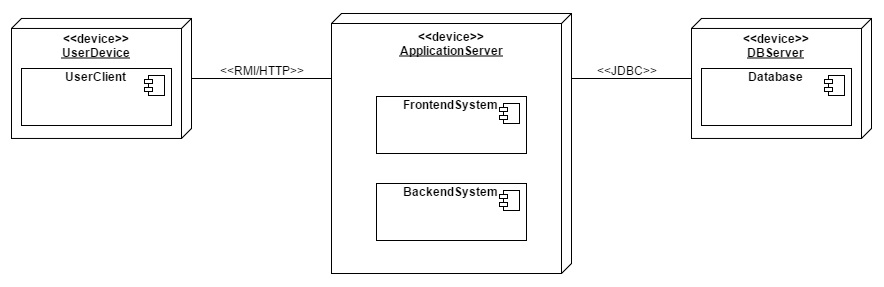
\includegraphics[width=0.9\linewidth]{../SE2_IMAGES/DeploymentDiagram}
				\caption{Deployment Diagram}
			\end{center}
		\end{figure}
	\end{landscape}
	\newpage
	\begin{landscape}
	\subsection{Runtime view}
		\begin{figure}[h!]
			\begin{center}
				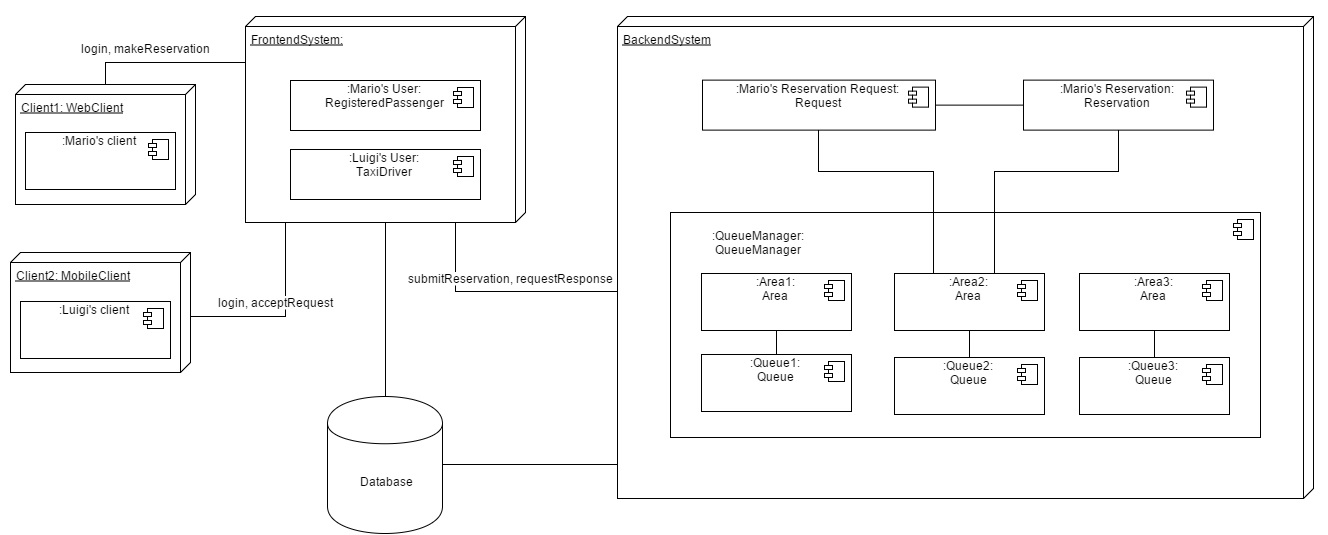
\includegraphics[width=0.9\linewidth]{../SE2_IMAGES/RuntimeDiagram}
				\caption{Runtime Diagram}
			\end{center}
		\end{figure}
	\end{landscape}
	\newpage
	\subsection{Component interfaces}
		\subsubsection{Guest}
		This is the basic interface assigned to client when the user accesses the application.
		It provides methods to perform all the operations that a "Guest" user can do:
		\begin{itemize}
			\item \textbf{register}: this method gives the possibility to an unregistered passenger to
			submit his personal data to perform a registration. If the registration succeeds, he will be
			stored in the database and will be able to log into the environment and be considered a registered passenger.
			\begin{description}
				\item[Input] Personal Data required for the registration
				\item[Output] The result of the registration (success or failure in case of error)
			\end{description}
			\item \textbf{login}: this method gives the possibility to login the environment to be considered
			a registered passenger. If this method succeeds, the Client will automatically substitute its Guest
			interface with a Registered Passenger interface related to the user that just performed the login.
			\begin{description}
				\item[Input] Login Data required for the login
				\item[Output] The result of the login (success or failure in case of error)
			\end{description}
			\item \textbf{makeRequest}: this method gives the possibility to a guest to make a single request.
			Some personal data and the consent for the automatic position recovery are required for the submission
			of the request. It also checks that all the constraints are respected before creating the Request object.
			\begin{description}
				\item[Input] Personal Data and consent
				\item[Output] Nothing is returned directly, but the client will receive notifications about the
				request status.
			\end{description}
		\end{itemize}
		\subsubsection{RegisteredPassenger}
		This interface substitutes the Guest one in the client when the login is successfully completed.
		It provides all the	functionalities that a Registered Passenger can exploit.
		\begin{itemize}
			\item \textbf{makeRequest}: like in the Guest, this method gives the possibility to make a single request.
			No personal data is required for the submission, because the system will automatically use the
			informations stored in the database during the registration process. This method also checks that
			all the constraints are respected before creating the Request object.
			\begin{description}
				\item[Input] Nothing
				\item[Output] Nothing is returned directly, but the client will receive notifications about the
				request status.
			\end{description}
			\item \textbf{makeReservation}: this method gives the possibility to a guest to make a single reservation.
			For a reservation some additional informations are required, that must be provided at the submission.
			This method also checks that all the constraints are respected before creating the Reservation object.
			\begin{description}
				\item[Input] The origin time and place where the taxi ride will begin
				\item[Output] Nothing is returned directly, but the client will receive notifications about the
				reservation and the consequent request statuses.
			\end{description}
		\end{itemize}
		\subsubsection{Request}
		This interface is provided to the User instances to create, and eventually interact, with a request.
		\begin{itemize}
			\item \textbf{makeRequest}: this method receives a User (a Guest o a RegisteredPassenger instance)
			and creates	an instance of a Request, launching also all the necessary processes to satisfy it.
			\begin{description}
				\item[Input] User
				\item[Output] A Request instance
			\end{description}
		\end{itemize}
		\subsubsection{Reservation}
		This interface is provided to the User instances to create, and eventually interact, with a reservation.
		\begin{itemize}
			\item \textbf{makeReservation}: this method receives a User (a Guest o a RegisteredPassenger instance)
			and the place and time informations necessary for the creation of a Reservation and instances a
			Reservation object, launching also all the necessary processes to satisfy it. This method fundamentally
			launches the makeRequest functionality at the right time.
			\begin{description}
				\item[Input] User, When and Where the request will take place
				\item[Output] A Reservation
			\end{description}
		\end{itemize}
	\subsection{Architectural styles and patterns}
	\subsection{Other design decisions}